% !TEX root = Bigall.tex
\section{Theoretische Grundlagen}
\subsection{Synthese von Nanopartikeln}
	Bei der Herstellung von Nanopartikeln wird zwischen der \glqq bottom-up\grqq - und der \glqq top-down\grqq - Methode unterschieden.
	Bei der \glqq top-down\grqq - Methode wird mit einem Festkörper angefangen, der dann durch verschiedene physikalische Zerkleinerungsmethoden auf eine gewünschte Partikelgröße gebrochen wird.
	Da diese Brüche nicht gleichmäßig stattfinden, eigenen sich diese Methoden nicht um monodisperse Nanokristalle herzustellen.
	Bei der \glqq bottom-up\grqq - Methode wird ein Nanopartikel aus vielen Monomeren zusammengesetzt, bis zur gewünschten Größe.
	Diese Methode kann mit einzelnen Klemmbausteinen verglichen werden, die zu größeren Gebilden zusammengesetzt werden können.
	Da man bei diesem Verfahren viele Parameter hat, die verändert werden können, durch die die Partikeleigenschaften eingestellt werden können, bietet sich das \glqq bottom-up\grqq - Verfahren zur Synthese monodisperser Partikel besser an.
	Parameter die eingestellt werden können sind u.a. Reaktionstemperatur und Dauer, Konzentration der Edukte, Druck oder Lösungsmittel.
	
	Die theoretische Beschreibung der Bildung monodisperser Nanopartikel geht auf Untersuchungen von LaMer und Dinegar zurück.\autocite{Lamer1950}
	Sie zeigten, dass die Bildung
	monodisperser Kolloide eine zeitlich diskrete (nicht kontinuierliche) Keimbildung
	erfordert, gefolgt von einem langsameren kontrollierten Wachstum der existierenden
	Kerne.
	Bei dem Konzept der sog. „schlagartigen Keimbildung“ muss demnach die
	Keimbildung zu einem einzigen Zeitpunkt ausgelöst werden. Weitere
	Keimbildungsereignisse sind auszuschließen. Startend in einer homogenen Phase setzt
	bei Überwindung der Energiebarriere die Keimbildung ein und es resultiert eine
	heterogene Phase unter homogener Nukleation. \autocite{Park2007}
	
	\begin{figure}[H]
		\centering
		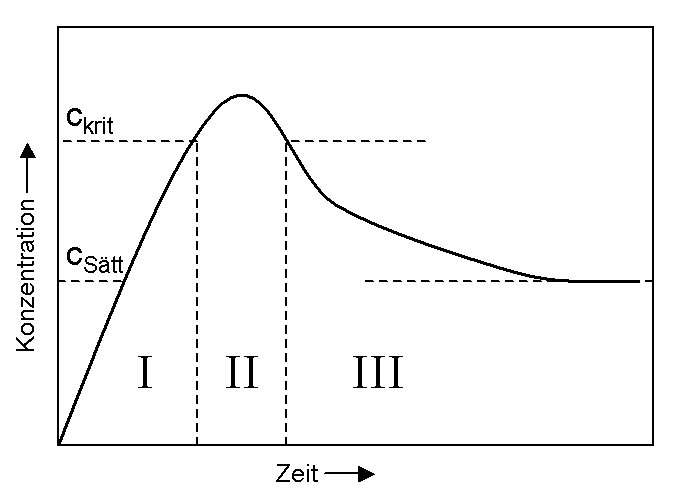
\includegraphics[width=0.6\textwidth]{Bilder/LaMer} 	
		\caption{LaMer-Diagramm: Monomerkonzentration als Funktion der Zeit nach.\autocite{Lamer1950}}
		\label{fig:LaMer}
	\end{figure}

	Im LaMer-Modell existieren 3 Stufen. 
	In Stufe I ist eine kontinuierliche Zunahme der Monomerkonzentration dargestellt.
	Durch die Energiebarriere kommt es auch nach Überschreiten der Sättigungs-Konzentration $C_{Sätt}$ zu keiner Keimbildung.
	Zum Erreichen der Keimbildung in Stufe II muss eine kritische Konzentration $c_{krit}$ überschritten werden.
	Hier werden schlagartig Keime gebildet mit einem kritischen Radius $r_{krit}$, wodurch die Monomerkonzentration wieder unter $c_{krit}$ sinkt, wo dann keine weiteren Keime mehr gebildet werden können.
	Hier wird dann Stufe III erreicht, bei der die Monomere nicht mehr zur Keimbildung, sondern zum Wachstum der Keime genutzt werden, bis ein Gleichgewichtszustand bei der Sättigungskonzentration erreicht wird.
	
%----------------------------------------------
	
	\subsection{Halbleiternanopartikel \& Größenquantisierungseffekt}
	Während Halbleiter als Festkörper eine feste Bandlücke zwischen Valenz- und Leitungsband aufweisen, ist sie bei Nanopartikeln eine von der Partikelgröße abhängige Eigenschaft.
	Allgemein gilt, dass bei kleineren Partikeln die Bandlücke zunimmt.
	\begin{figure}[h]
		\centering
		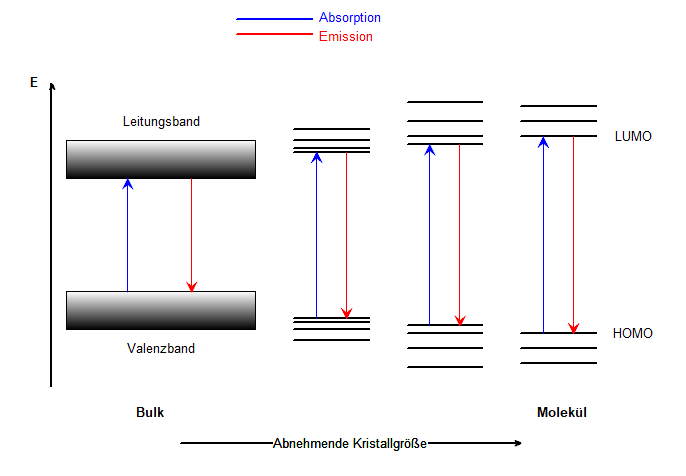
\includegraphics[width=0.6\linewidth]{Bilder/Quantumsizeeffect}
		\caption{Schematische Darstellung der Veränderung der Bandlücke bei abnehmender Kristallgröße.}
		\label{fig:LCAO}
	\end{figure}
	
    Dies lässt sich über 2 Theorien beschreiben. Zum einen auf der Basis des LCAO-Modells (Linear Combination of Atomic Orbitals) bei dem Nanopartikel als große Moleküle gesehen werden, zum anderen auf Basis der Festkörpertheorie, die Nanopartikel als kleine Festkörper beschreibt.
	
	Bei der LCAO-Methode bilden n Atomorbitale, die gleiche Symmetrie und ähnliche Energie besitzen, durch lineare Kombination, n Molekülorbitale. Wird n sehr groß, kommt es zu einer großen Anzahl Energieniveaus, die sehr nahe beieinander liegen, wodurch kontinuierliche Energiebänder entstehen. Bei Isolatoren und Halbleitern gibt es eine Bandlücke zwischen den Bändern, die bei großen Festkörpern, bei denen die Annahme $n \rightarrow \infty$  gilt, zu einer festen Materialeigenschaft führt. Bei Nanopartikeln gilt diese Näherung allerdings nicht mehr, wodurch sich die kontinuierlichen Bänder mit sinkender Anzahl Atomen wieder in diskrete Energieniveaus aufteilen. Dabei vergrößert sich auch die Bandlücke wieder, wie in \cref{fig:LCAO} dargestellt.
	
	Die Festkörpertheorie: Kommt es zur Absorption eines Photons, kommt es zu einem Loch $h^{+}$  im Valenzband und zu einem Elektron $e^{-}$ im Leiterband, die jedoch aufgrund ihrer Polarität, sich nicht frei im Kristall bewegen können und so ein Paar, das Exziton genannt wird, bilden. Der durchschnittliche Abstand von $e^{-}$ und $h^{+}$ wird Exziton-Bohr-Radius genannt. In einem Nanopartikel ist die Bewegung durch die Partikelgrenzen beschränkt, die als Potentialgrenzen wirken, ähnlich des „Teilchen im Kasten“-Modells, bei dem das Potential außerhalb unendlich ist.
	Ist die Partikelgröße kleiner als der Exziton-Bohr-Radius, muss somit die Bandlücke steigen.
	Da ein kristalliner Festkörper kein konstantes Potential aufweist, sondern eher ein periodisch oszillierendes, wird die Effektive-Masse-Näherung angewandt, bei der sowohl $e^{-}$ als auch $h^{+}$ eine effektive Masse zugeordnet wird, die als Maß für Mobilität der Ladungsträger angesehen werden kann. Daraus ergibt sich die BRUS-Formel:
	\begin{equation}
	\label{eq:BRUS}
	E_{NC}=E_{g}+\frac{h^{2}}{8R^{2}}\left( \frac{1}{m^{*}_{e}}+\frac{1}{m^{*}_{h}}\right)-\frac{1,8e^{2}}{4\pi\epsilon_{0}\epsilon_{r}R} 
	\end{equation}
	\begin{multicols}{2}
		\begin{flushleft}
			$E_{NC}$:	Bandlücke des Nanokristalls\\
			$E_{g}$:	Bandlücke des Festkörpers\\
			$h$:		Plank´sches Wirkungsquantum\\
			$R$:		Partikelgröße\\
			$m^{*}_{e}$: Effektive Masse des $e^{-}$\\
			$m^{*}_{h}$: Effektive Masse des $h^{+}$\\
			$\epsilon_{0}$: Permittivität des Vakuums\\
			$\epsilon_{r}$: relative Permittivität\\
			$e$: Elementarladung\\
		\end{flushleft}
	\end{multicols}
	
%-----------------------------------------------------

    \subsection{Metallnanopartikel \& Plasmonik}
    
    \subsection{Metall-Halbleiter-Nanopartikel}
    
    \subsection{Nanopartikelbasierte Gele}
    
    \subsection{Edelmetallgele}
    
    \subsection{Metall-Halbleiter-Gele}